\documentclass[12pt]{article}
\usepackage{amsmath,amssymb,physics,geometry,hyperref,listings,xcolor,graphicx,booktabs,float}
\geometry{margin=1in}
\hypersetup{colorlinks=true, linkcolor=blue, citecolor=blue, urlcolor=blue}
\graphicspath{{docs/}}

\definecolor{codebg}{RGB}{18,22,28}
\definecolor{codekw}{RGB}{99,179,237}
\definecolor{codestr}{RGB}{236,201,75}
\definecolor{codecom}{RGB}{136,192,112}
\definecolor{codeid}{RGB}{229,231,235}

\lstdefinelanguage{GLSL}{
  morekeywords={float,int,bool,vec2,vec3,vec4,mat2,uniform,in,out,return,for,if,else,struct,void},
  sensitive=true,
  morecomment=[l]{//},
  morecomment=[s]{/*}{*/},
  morestring=[b]"
}

\lstset{
  language=GLSL,
  backgroundcolor=\color{codebg},
  basicstyle=\ttfamily\small\color{codeid},
  keywordstyle=\color{codekw}\bfseries,
  stringstyle=\color{codestr},
  commentstyle=\color{codecom}\itshape,
  numbers=left,
  numberstyle=\tiny\color{gray},
  stepnumber=1,
  numbersep=10pt,
  showstringspaces=false,
  breaklines=true,
  frame=single,
  rulecolor=\color{black},
  tabsize=2
}

\title{Geodesica: Real-Time Schwarzschild Black Hole Rendering via GPU-Side Geodesic Integration}
\author{Aanish Farrukh\\Independent / FarrukhCorp}
\date{\today}

\begin{document}
\maketitle

\begin{abstract}
Geodesica is a real-time black hole renderer written in TypeScript, WebGL2, and GLSL ES 3.00. The simulator visualizes a Schwarzschild black hole by integrating null geodesics per pixel directly inside a fragment shader, rather than relying on precomputed lookup textures or offline ray tracing. Its core numerical method is fourth-order Runge--Kutta (RK4) integration of an equivalent Cartesian form of the Schwarzschild photon orbit equation, allowing the program to produce gravitational lensing, a photon ring, multi-crossing accretion-disk accumulation, gravitational redshift, relativistic Doppler amplification, and observer aberration in real time. The rendering pipeline is organized as a two-pass system: a high-dynamic-range geodesic pass writes to a floating-point framebuffer, followed by bloom, ACES filmic tone mapping, and vignette post-processing. This paper documents the physical model actually implemented in the simulator, the numerical approximations required for interactive performance, and the places where the renderer intentionally simplifies real black hole astrophysics in order to remain responsive in the browser.
\end{abstract}

\section{Introduction}
The Schwarzschild solution is the simplest exact black hole spacetime in general relativity: static, spherically symmetric, and non-rotating. Even this ``minimal'' black hole produces visually rich optical effects, including strong gravitational lensing, a bright photon ring, and dramatic distortions of a surrounding accretion flow.

Black hole visualization has a long history. Luminet's 1979 paper produced one of the first physically motivated images of a black hole with a thin accretion disk \cite{luminet1979}. More recently, the rendering work behind \emph{Interstellar} demonstrated how cinematic black hole imagery could still be grounded in relativistic ray tracing \cite{james2015}. Web-based real-time visualizers such as \texttt{schwarzschild} by rantonels \cite{rantonels} and \texttt{black-hole} by oseiskar \cite{oseiskar} showed that browser GPU pipelines can support interactive black hole rendering.

Geodesica differs from offline renderers by integrating geodesics on the GPU for every visible pixel at interactive frame rates. Rather than tracing rays on the CPU or relying on precomputed lensing maps, the simulator runs a fragment-shader RK4 integrator in real time. That design keeps the system interactive while still preserving the dominant visual signatures of Schwarzschild spacetime.

\begin{figure}[htbp]
\centering
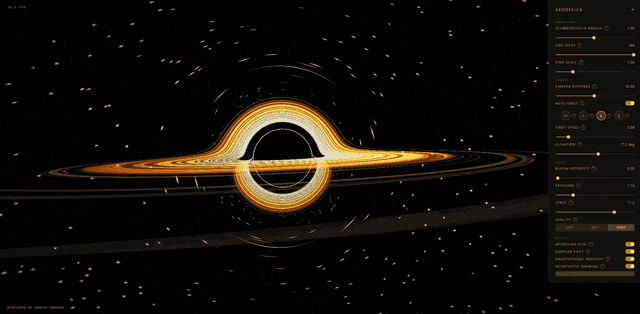
\includegraphics[width=\linewidth]{preview.jpg}
\caption{A representative frame from Geodesica showing the lensed accretion disk, photon ring, procedural star background, and interactive control panel.}
\label{fig:preview}
\end{figure}

\section{The Schwarzschild Spacetime}
In geometric units, the Schwarzschild metric is
\begin{equation}
ds^2 = -\left(1 - \frac{r_s}{r}\right) dt^2 + \left(1 - \frac{r_s}{r}\right)^{-1} dr^2 + r^2 d\Omega^2,
\label{eq:schwarzschild_metric}
\end{equation}
where
\begin{equation}
r_s = \frac{2GM}{c^2}
\label{eq:schwarzschild_radius}
\end{equation}
is the Schwarzschild radius. The event horizon lies at
\begin{equation}
r = r_s,
\label{eq:event_horizon}
\end{equation}
the photon sphere lies at
\begin{equation}
r = \frac{3}{2} r_s,
\label{eq:photon_sphere}
\end{equation}
and the innermost stable circular orbit (ISCO) for massive particles lies at
\begin{equation}
r = 3 r_s.
\label{eq:isco}
\end{equation}

Geodesica exposes $r_s$ as a user control and uses it as the master scale for the event horizon, the photon-ring highlighting term, and the disk geometry. The disk itself is rendered from $3r_s$ outward, matching the ISCO-based inner edge used in the shader.

\section{Null Geodesics and the Photon Orbit Equation}
For null geodesics in Schwarzschild spacetime, the conserved energy $E$ and angular momentum $L$ give the effective radial equation
\begin{equation}
\left(\dv{r}{\lambda}\right)^2 + V_{\mathrm{eff}}(r) = E^2,
\label{eq:effective_potential}
\end{equation}
with photon effective potential
\begin{equation}
V_{\mathrm{eff}}(r) = \left(1 - \frac{r_s}{r}\right)\frac{L^2}{r^2}.
\label{eq:photon_potential}
\end{equation}

Introducing $u = 1/r$ and using the azimuthal angle $\phi$ as the orbit parameter yields the standard photon orbit equation
\begin{equation}
\dv[2]{u}{\phi} + u = \frac{3}{2} r_s u^2,
\label{eq:photon_orbit}
\end{equation}
which appears as Eq.~25.40 in Misner, Thorne, and Wheeler \cite{mtw}.

Geodesica does \emph{not} integrate Eq.~\eqref{eq:photon_orbit} directly in $(u,\phi)$ form. Instead, the fragment shader uses an equivalent Cartesian central-force form derived from the same Schwarzschild correction:
\begin{equation}
\frac{d^2 \mathbf{r}}{d\lambda^2} = -\frac{3}{2} r_s h^2 \frac{\mathbf{r}}{\norm{\mathbf{r}}^5},
\label{eq:cartesian_force}
\end{equation}
where $h^2 = \norm{\mathbf{r} \times \mathbf{v}}^2$ is the squared specific angular momentum of the ray. This form is convenient for GPU execution because each pixel can evolve a ray state $(\mathbf{r}, \mathbf{v})$ without solving coordinate singularities in angular variables.

\section{Numerical Integration: RK4 on the GPU}
Explicit Euler integration is cheap, but it accumulates visible trajectory error rapidly in strong-curvature regions near the photon sphere. Geodesica therefore uses classical fourth-order Runge--Kutta integration. For a state $\mathbf{y}$ satisfying $\dot{\mathbf{y}} = f(\mathbf{y})$, RK4 updates via
\begin{align}
\mathbf{k}_1 &= f(\mathbf{y}_n), \\
\mathbf{k}_2 &= f\!\left(\mathbf{y}_n + \frac{\Delta t}{2}\mathbf{k}_1\right), \\
\mathbf{k}_3 &= f\!\left(\mathbf{y}_n + \frac{\Delta t}{2}\mathbf{k}_2\right), \\
\mathbf{k}_4 &= f\!\left(\mathbf{y}_n + \Delta t\,\mathbf{k}_3\right), \\
\mathbf{y}_{n+1} &= \mathbf{y}_n + \frac{\Delta t}{6}\left(\mathbf{k}_1 + 2\mathbf{k}_2 + 2\mathbf{k}_3 + \mathbf{k}_4\right).
\label{eq:rk4}
\end{align}

In Geodesica, every fragment stores the ray position and direction in a \texttt{RayState} struct and advances it in the fragment shader. The current implementation allows 32 to 256 user-selected ODE steps, with quality presets mapped to 64, 128, and 256 steps. The renderer also scales step size with both camera distance and quality preset, so higher quality means more steps and smaller steps.

The actual GLSL integrator is compact enough to run directly per pixel:

\begin{lstlisting}
RayDeriv geodesicDeriv(RayState state) {
  float r = max(length(state.pos), EPSILON);
  vec3 angularMomentum = cross(state.pos, state.vel);
  float h2 = dot(angularMomentum, angularMomentum);
  float r2 = r * r;
  float r5 = max(r2 * r2 * r, EPSILON);
  float coeff = -1.5 * uSchwarzschildRadius * h2 / r5;
  RayDeriv deriv;
  deriv.dPos = state.vel;
  deriv.dVel = state.pos * coeff;
  return deriv;
}

RayState rk4Step(RayState state, float dt) {
  RayDeriv k1 = geodesicDeriv(state);
  RayDeriv k2 = geodesicDeriv(applyDeriv(state, k1, dt * 0.5));
  RayDeriv k3 = geodesicDeriv(applyDeriv(state, k2, dt * 0.5));
  RayDeriv k4 = geodesicDeriv(applyDeriv(state, k3, dt));

  state.pos += (k1.dPos + 2.0 * k2.dPos + 2.0 * k3.dPos + k4.dPos) * (dt / 6.0);
  state.vel += (k1.dVel + 2.0 * k2.dVel + 2.0 * k3.dVel + k4.dVel) * (dt / 6.0);
  state.vel = normalize(state.vel);
  return state;
}
\end{lstlisting}

Because this work happens inside the fragment shader, each output pixel independently ray-marches through the Schwarzschild field. This is the core reason the simulator remains interactive: the browser GPU runs thousands of geodesic integrations in parallel.

\section{The Accretion Disk}
Thin-disk theory provides the astrophysical backdrop for Geodesica's disk model. In the Shakura--Sunyaev picture, the effective temperature scales approximately as
\begin{equation}
T(r) \propto \left[\frac{1}{r^3}\left(1 - \sqrt{\frac{r_i}{r}}\right)\right]^{1/4},
\label{eq:thin_disk_temperature}
\end{equation}
with $r_i$ the inner edge of the disk \cite{shakura1973}. A more complete radiative transfer model would map this temperature to color using a blackbody spectrum.

Geodesica uses that theory as inspiration, but the implemented shader is intentionally simpler. The disk is represented as a geometrically thin tilted annulus with inner radius $3r_s$ and outer body radius $14r_s$, plus spiral-arm structure extending to $22r_s$. Rather than evaluating Eq.~\eqref{eq:thin_disk_temperature} explicitly, the shader uses a hand-tuned radial color gradient, vertical density falloff, and procedural modulation terms:
\begin{itemize}
\item a radial emissivity ramp from bright yellow-white near the inner disk to dark red-brown farther out,
\item fractal Brownian motion (FBM) for fiber-like turbulent texture,
\item a spiral-arm modulation for coherent rotating structure,
\item exponential vertical attenuation to keep the disk thin,
\item explicit annulus masking to preserve the disk silhouette.
\end{itemize}

Differential rotation is encoded by phase terms proportional to
\begin{equation}
\omega(r) \propto r^{-3/2},
\label{eq:keplerian_rotation}
\end{equation}
which matches the Keplerian scaling used in thin-disk intuition. When a ray crosses the tilted disk plane multiple times, Geodesica accumulates contributions from each intersection, reducing transparency by a fixed factor after each hit. That gives the disk visible depth without resorting to volumetric simulation.

\section{Relativistic Visual Effects}
\subsection{Gravitational Lensing}
The lensing effect in Geodesica emerges directly from the RK4 geodesic integration. Each fragment launches a ray from the camera, bends it according to Eq.~\eqref{eq:cartesian_force}, and then samples the background using the final deflected direction. Strong lensing appears automatically near the hole, while the bright photon ring is emphasized with an additional glow term based on periapsis distance to the photon sphere:
\begin{equation}
I_{\mathrm{ring}} \propto \exp\!\left[-\frac{(r_{\min} - 1.5r_s)^2}{\sigma^2}\right].
\label{eq:photon_ring_glow}
\end{equation}

\subsection{Doppler Beaming}
For disk emission, the shader uses the relativistic Doppler factor
\begin{equation}
D = \sqrt{\frac{1+\beta}{1-\beta}},
\label{eq:doppler_factor}
\end{equation}
where $\beta$ is the line-of-sight velocity in units of $c$. Disk intensity is scaled approximately as
\begin{equation}
I \propto D^4,
\label{eq:doppler_intensity}
\end{equation}
which strongly brightens the approaching side and dims the receding side. The orbital speed approximation used in the shader is
\begin{equation}
\frac{v}{c} \approx \sqrt{\frac{r_s}{2r}}.
\label{eq:keplerian_beta}
\end{equation}
This is the dominant reason one side of the disk appears dramatically brighter.

\subsection{Gravitational Redshift}
Gravitational redshift is modeled using
\begin{equation}
1 + z = \frac{1}{\sqrt{1 - r_s/r}}.
\label{eq:grav_redshift}
\end{equation}
In practice, Geodesica converts this into a scalar dimming and a warmer color balance near the hole. The effect is intentionally simplified: it is not a full spectral transport calculation, but it does convey the expected visual darkening and reddening of emission close to the horizon.

\subsection{Relativistic Aberration}
The simulator also supports an observer-motion mode. The scene controller estimates observer velocity from keyboard-driven camera translation, and the fragment shader applies an aberration transform to the outgoing ray direction before tracing. This shifts the apparent sky position of stars and affects the brightness of the sampled background, producing a plausible motion-induced relativistic distortion.

\section{Rendering Pipeline}
Geodesica targets WebGL2 with GLSL ES 3.00. The main reasons for choosing WebGL2 over WebGL1 are support for modern shader syntax and floating-point render targets through \texttt{EXT\_color\_buffer\_float}.

The renderer uses a two-pass pipeline:
\begin{enumerate}
\item A geodesic pass traces the black hole scene into an \texttt{RGBA16F} framebuffer.
\item A post-processing pass applies bloom, exposure, ACES filmic tone mapping, gamma correction, and vignette before presenting to the canvas.
\end{enumerate}

Bloom is implemented with a bright-pass threshold and a compact multi-tap blur at two radii. Tone mapping uses the ACES filmic curve,
\begin{equation}
\mathrm{ACES}(x) = \mathrm{clamp}\!\left(\frac{x(2.51x + 0.03)}{x(2.43x + 0.59) + 0.14}, 0, 1\right),
\label{eq:aces}
\end{equation}
which compresses the HDR image into display space while preserving highlight structure better than a linear exposure alone.

The background star field is also procedural. No external texture skybox is used in the current simulator; instead, multiple star layers are synthesized with hashed spherical UV cells and simple color-category selection in the shader.

\section{Where the Simulation Simplifies Reality}
Several simplifications are deliberate:
\begin{itemize}
\item Only the Schwarzschild metric is implemented; there is no Kerr spin term.
\item The accretion disk is geometrically thin and does not model full vertical structure.
\item Disk turbulence is procedural FBM, not magnetohydrodynamic simulation.
\item Disk color is a stylized emissivity ramp, not a full blackbody spectrum computed from Eq.~\eqref{eq:thin_disk_temperature}.
\item Background stellar spectra are approximated procedurally.
\item Lower ODE step counts and larger step sizes introduce visible lensing error.
\item Polarization is not modeled.
\item The renderer is monochromatic in the sense of display RGB only; it does not simulate multi-wavelength channels such as X-ray or radio bands.
\item The photon ring is enhanced with an explicit glow term for readability.
\end{itemize}

These simplifications are acceptable for an interactive browser renderer, but they should not be confused with a high-fidelity astrophysical transport code.

\section{Performance}
The fragment-shader RK4 integration dominates frame time. That cost scales roughly linearly with the number of ODE steps, and in Geodesica the quality presets also change step size, making the high preset both more accurate and more expensive. The browser renderer further limits device pixel ratio to 2 in order to avoid runaway fill-rate cost on high-density displays.

Table~\ref{tab:performance} gives illustrative step-count scaling. These values are not hard benchmarks baked into the repository; they are approximate desktop-class estimates meant to communicate the trade-off between speed and fidelity.

\begin{table}[htbp]
\centering
\caption{Illustrative step-count scaling in Geodesica.}
\label{tab:performance}
\begin{tabular}{@{}lll@{}}
\toprule
Steps & Approx.\ frame time & Photon ring accuracy \\
\midrule
32  & $\sim$2 ms  & Poor \\
64  & $\sim$4 ms  & Acceptable \\
128 & $\sim$8 ms  & Good \\
256 & $\sim$16 ms & Excellent \\
\bottomrule
\end{tabular}
\end{table}

The quality preset system maps directly onto the user interface:
\begin{itemize}
\item \texttt{low}: 64 steps,
\item \texttt{med}: 128 steps,
\item \texttt{high}: 256 steps.
\end{itemize}
On mobile hardware, reducing steps, bloom intensity, and star density is the most direct way to preserve responsiveness.

\section{Conclusion}
Geodesica demonstrates that a browser-based renderer can produce convincing Schwarzschild black hole imagery in real time without precomputed textures or offline ray tracing. Its core contribution is straightforward but effective: each fragment integrates a null geodesic using RK4 on the GPU, then shades the disk and background from the resulting trajectory. On top of that core, the simulator layers Doppler boosting, gravitational redshift, observer aberration, HDR post-processing, and interactive camera controls.

Compared with prior real-time browser projects such as rantonels' \texttt{schwarzschild} \cite{rantonels} and oseiskar's \texttt{black-hole} \cite{oseiskar}, Geodesica emphasizes a self-contained procedural pipeline with a stylized but physically motivated disk and explicitly documented implementation trade-offs. Natural future directions include Kerr geodesics, polarization, more faithful spectral transport, and disk models informed by MHD rather than procedural turbulence.

\begin{thebibliography}{9}
\bibitem{mtw}
Misner, C.~W., Thorne, K.~S., Wheeler, J.~A. (1973).
\textit{Gravitation}.
W.~H. Freeman.

\bibitem{luminet1979}
Luminet, J.-P. (1979).
Image of a spherical black hole with thin accretion disk.
\textit{Astronomy and Astrophysics}, 75, 228--235.

\bibitem{james2015}
James, O., von Tunzelmann, E., Franklin, P., Thorne, K.~S. (2015).
Gravitational lensing by spinning black holes in astrophysics, and in the movie \textit{Interstellar}.
\textit{Classical and Quantum Gravity}, 32(6).

\bibitem{shakura1973}
Shakura, N.~I., Sunyaev, R.~A. (1973).
Black holes in binary systems. Observational appearance.
\textit{Astronomy and Astrophysics}, 24, 337--355.

\bibitem{rantonels}
rantonels. (2015).
\textit{schwarzschild: A real-time WebGL visualization of a Schwarzschild Black Hole}.
GitHub. \url{https://github.com/rantonels/schwarzschild}

\bibitem{oseiskar}
oseiskar. (2016).
\textit{black-hole: WebGL simulation of a Schwarzschild black hole}.
GitHub. \url{https://github.com/oseiskar/black-hole}
\end{thebibliography}

\end{document}
